%!TEX root = ../main.tex
In this chapter, we will explain our implementation choices and the tools we used to carry out our project. Our main goal was to release a maintainable open source library so that other developers could use it and contribute to it. Our choices were mainly guided by this goal.

\section{Langage choice}

\begin{wrapfigure}[7]{r}{3.5cm}
	\vspace{-8mm}
	
\includegraphics[width =2cm]{images/Java_logo.png}
	\captionof{figure}{Java Logo}
\end{wrapfigure}

In order to implement the different flow algorithms presented, we had to choose a programming language. We decided to develop the different algorithms with \textbf{Java}\footnote{https://community.oracle.com/community/java}. Java is a programming language created in 1995 by Sun Microsystems. Java is designed to run acress multiple operating systems, including Linux, Mac OS X and Windows. Java is known to be flexible, scalable and maintainable. Java is an object-oriented programming language, which permits the development of modulable applications via systems like encapsulation, composition, inheritance, and delegation. We choose Java because of the followings reasons:
\begin{itemize}
	\item Java is very popular. This is a key point because we want that the librairies we developped were accessible to as many. Another consequence of this is that Java is well documented.
	\item Java is modulable. The OO Java paradigm is useful to develop this project were different algorithms and different data structures must be implemented. Concepts like inheritance, interfaces are very useful to achieve this.
	\item Java is fast. Many optimizations have improved the performance of the JVM over time such as the Just-in-time compiling. Some of our instance are very big, so we need a language able to solve them quickly.
	\item We are accustomed to using java. A good knowledge of the language is required to make correct implementations.
\end{itemize}


\section{Structure}

Our project is divided in two core packages: \textit{models} and \textit{solvers}. The first one, is contains all the representations of the network we used. The second contains all the different algorithms we implemented. There is two others packages: \textit{objects} which contains implementation of some data structures and \textit{results} which contains instance generators and results analyzers.

\subsection{Package: Models}

This package contains all the network representation we implemented: \textit{SplitArrayGraph}, \textit{SparseMapGraph}, \textit{TreeMapGraph}, \textit{LinkedListGrah} and \textit{HashMapGraph}. As we can see in the Figure~\ref{img:models}, all these class implements the interface \textit{Graph} which define the behaviour of the object that represent the network. Here is the method which must be implemented when creating a network representation in our project:
\begin{description}
	\item[\texttt{parse(file\_path)}] parse the file given in the constructor argument. The parse method must take into account if the graph is directed or not;
	\item[\texttt{getV(), getE()}] return respectively the number of vertices and the number of edges;
	\item[\texttt{getVertex(id)}] return the vertex with the corresponding id;
	\item[\texttt{getVertices()}] return the set of vertices;
	\item[\texttt{getAdjacents(id)}] return the neighbours of the vertex \textit{id};
	\item[\texttt{removeEdge(id1, id2)}] remove the edge between \textit{id1} and \textit{id2};
	\item[\texttt{addEdge(id1, id2, c)}] add an edge from \textit{id1} to \textit{id2} with the capacity \textit{c};
	\item[\texttt{getCapacity(id1, id2)}] return the capacity of the edge between \textit{id1} and \textit{id2};
	\item[\texttt{setCapacity(id1, id2, c)}] set the capacity of the edge between \textit{id1} and \textit{id2} at \textit{c};
	\item[\texttt{getAdjacentsSize(id)}] return the number of neighbours of the vertex \textit{id};
	\item[\texttt{getMaxCapacity()}] return the biggest capacity in the network: used to initalize the scaling phase.
\end{description}

We defined the abstract class \textit{SimpleGraph} which contains all the common code between all the network representations we implemented. 

\begin{figure}
\centering
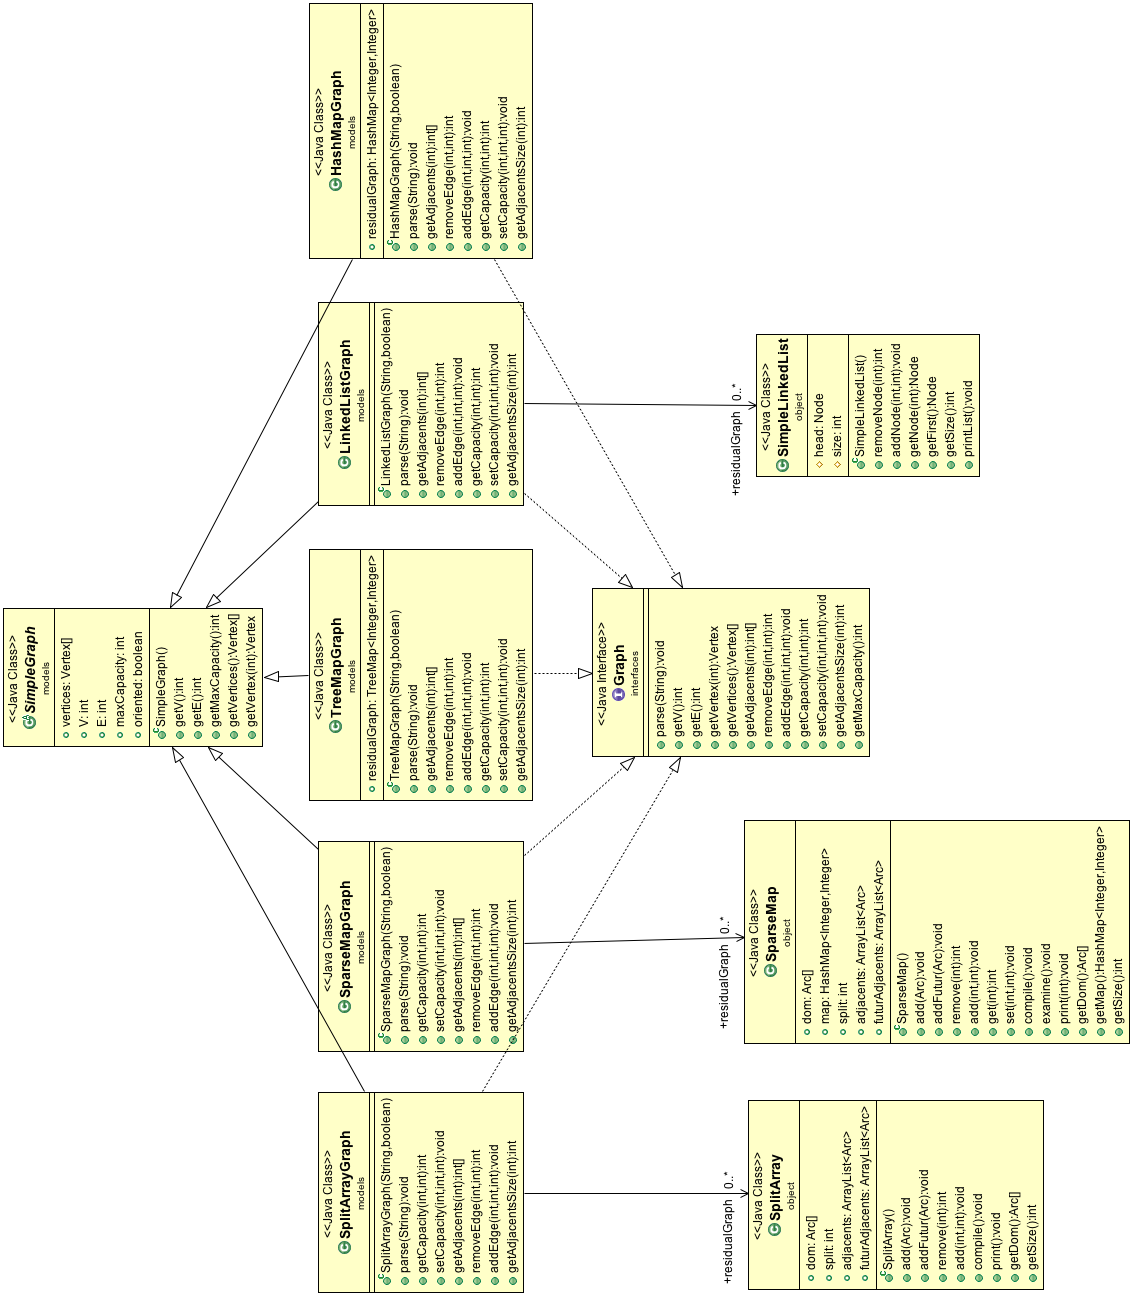
\includegraphics[scale=0.45]{images/models_diagram.png}
\caption{UML diagram of the package models.}
\label{img:models}
\end{figure}

\subsection{Package: Solvers}
 This package contains all the solvers we implemented. As we said in the Chapter 2, there is two family of algorithm to solve the maximum flow problem: the augmenting path algorithms and the preflow-push algorithms. The different algorithms in the augmenting path have a lot in common. For example, the difference between the Ford-Fulkerson algorithm and the Edmonds-Karp algorithm is how the algorithm find an augmenting path.  As we can see in the Figure~\ref{img:solver}, we used the strength of inheritance to avoid duplicate code. On the other part, the preflow-push algorithm have a lot of differences in their implementations, we decided split them in three classes.


\begin{figure}
\centering
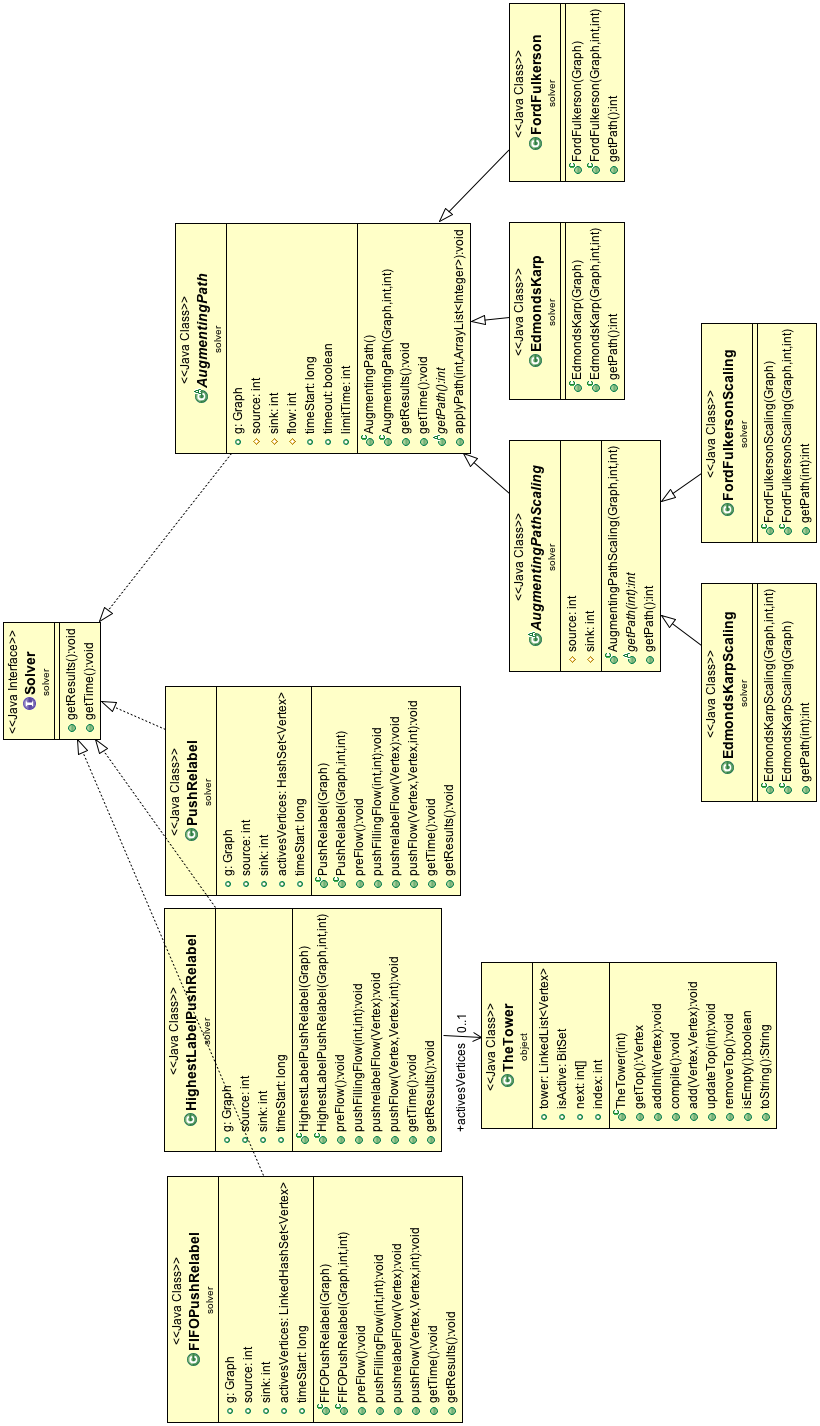
\includegraphics[scale=0.5]{images/solver_diagram.png}
\caption{UML diagram of the package solver.}
\label{img:solver}
\end{figure}

The solvers have a constructor overloading, which permits to define any vertex as the \textit{source} and the \textit{sink}.

\subsection{Package: Objects}

This package contains several data structures: 
\begin{description}
	\item[\texttt{Vertex.java}] used to represent a vertex;
	\item[\texttt{Arc.java}] used to represent an arc;
	\item[\texttt{Edge.java}] used to represent an edge. The difference between an arc and an edge is that the arc does not have the information about the origin vertex;
	\item[\texttt{SimpleLinkedList.java}] implementation of a linked list;
	\item[\texttt{Node.java}] represent a node in a linked list;
	\item[\texttt{SplitArray.java}] implementation of the split array;
	\item[\texttt{SparseMap.java}] implementation of the sparse map;
	\item[\texttt{TheTower.java}] data structure used to select the highest label in the highest label preflow-push algorithm.
\end{description}

\subsection{Package: Results}

This small package contains four classes. The first are the instances generators: \textit{InstanceGeneratorDensity.java} and \textit{InstanceGeneratorSize.java}. The first class generate an instance with different densities and the second with different sizes. The two last classes are \textit{ResultsConverterByDensity.java} and \textit{ResultsConverterBySize.java}. They are used to analyze our results.

\subsection{Conclusion}


The main advantage of our structure is how easy is to add different data structures or solvers. All you need is to implement the interfaces and add your own class in the correct package. Then, the solvers can be call with different data structures with a few line of codes as we can see in the Figure~\ref{simple_code}. Another advantage is that our code can be used as a library, without even looking at the code of it.

\begin{figure}
\begin{lstlisting}
Graph sm = new SparseMapGraph("file_path", true);
Solver ek = new EdmondsKarp(sm);
ek.getResults();
Solver pr = new PushRelabel(sm);
pr.getResults();
\end{lstlisting}
\caption{Example of use.}
\label{simple_code}
\end{figure}

\section{Collecting and displaying results}

%% How we launch script to get results

\begin{figure}
\centering
\begin{subfigure}{.5\textwidth}
  \centering
  
\includegraphics[width=.4\linewidth]{images/pythonlogo.png}
  \caption{Python Logo}
  \label{fig:python}
\end{subfigure}%
\begin{subfigure}{.5\textwidth}
  \centering
  
\includegraphics[width=.4\linewidth]{images/rlogo.jpg}
  \caption{R Logo}
  \label{fig:r}
\end{subfigure}
\label{fig:logos}
\end{figure}


In order to gather the different run times of all the algorithm we implemented on all the instances we generated, we decided to automate the launch of the different algorithms. We decided to make a script in \textbf{Python}\footnote{https://www.python.org} because it was the easiest way to do it. The Python script launch the different algorithms with the different data structes on all the instance, and store the computations time collected on a text file. A Java program is then used to classify the run times by solver and by instance and store these results in a csv file.
When we have the run times in the right form, we use the library \textbf{ggplot2}\footnote{http://ggplot2.org} of the \textbf{R}\footnote{https://www.r-project.org} language to plot the different graphs. We choosed this library because the graphs rendered are very customizable and  very nice.

\section{Tools}

\subsection{Version control system}

\begin{wrapfigure}[4]{r}{3.5cm}
	\vspace{-5mm}
	
\includegraphics[width =2cm]{images/Git-logo.png}
	\captionof{figure}{Git Logo}
\end{wrapfigure}

Using a versioning tool appeared to us from the beginning as an evidence. Our main needs were to share the code we did between us and to version it. We decided to use \textbf{Git}\footnote{https://git-scm.com} because we already both master it and it is one of the most popular versioning tool. We used \textbf{Github}\footnote{https://github.com} to host our application. With Github, it is fearly easy to make our project open source and knowing that this platform is very popular among developers, our project can benefit from a certain visibility. Our repository can be found at the following url: \url{https://github.com/denisgenon/flow_algorithm}.

\subsection{Management application}

\begin{wrapfigure}[4]{r}{3.5cm}
	\vspace{-5mm}
	
\includegraphics[width =2cm]{images/Trello_Logo.png}
	\captionof{figure}{Trello Logo}
\end{wrapfigure}


Even if we were only two working on the project, we judged useful to have project management tool to assist us. This kind of tools permits us to separate the tasks to make, to write somewhere our ideas, to fix deadlines and to see the evolution of our project. We decided to use \textbf{Trello}\footnote{https://trello.com} because we were already used to it. Trello uses the kanban paradigm for managing projects. Our project were represented as a board, which contains columns corresponding to some states (backlog, nice to have, in progress, \dots). Each column contains lists of cards which were our tasks. In this way, we could follow the flow of a feature from idea to implementation.

